% Author: Glen Newton
%
% Copyright 2010-2015 Glen Newton newtong@acm.org
%
% Creative Commons Attribution-NonCommercial-ShareAlike 2.5 Canada
% License. http://creativecommons.org/licenses/by-nc-sa/2.5/ca/
%
% See d_afterMichel1997.tex on how to build
%
%

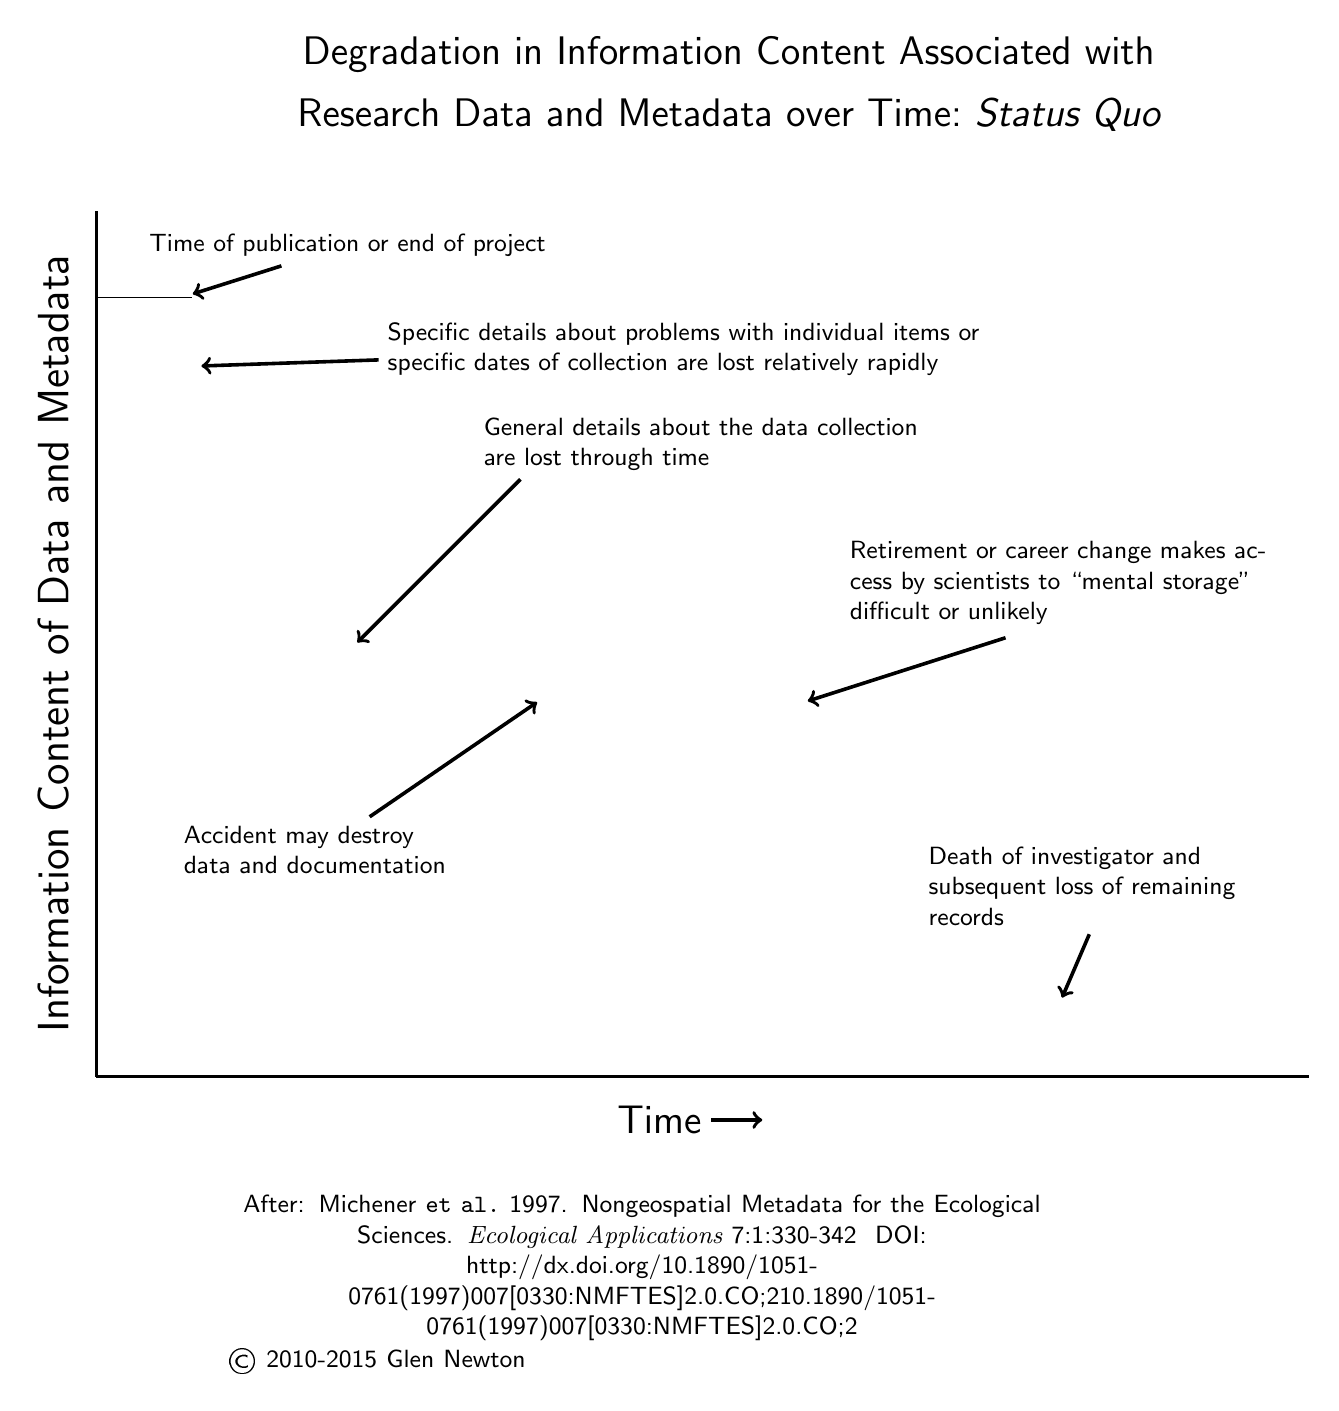
\begin{tikzpicture}[domain=0:14, scale=1.1]
  \draw[line width=1.3pt] (0,0) -- (0,10);
  \draw[line width=1.3pt] (0,0) -- (14,0);
  \sffamily


  %%%%%%%%%%%%%%%%%%%%%%%%%%%%%%% 
  \draw (0,9) -- (1.1,9);
  \node (pub) at ( 1,9) {};
  \node (pubtext) at (2.9,9.6) {\small  Time of publication or end of project};
  \draw[->,line width=1.3pt] (pubtext) -- (pub);
  
  
  %%%%%%%%%%%%%%%%%%%%%%%%%%%%%%% 
  \draw[domain=1.1:8.1,smooth] plot function{4+ ((1 / (.5*(x-0.7))))};
  \draw[domain=1.1:7] plot[id=x] function{9+1/x^2} ;
  
  \node (loss0) at ( 1.1,8.2) {};
  {\small 
    \node[text width=8cm] (loss0text) at (7,8.4) 
    % \node(loss0text) at (12,8.4) 
    {
      Specific details about problems with individual items or 
      specific dates of collection are lost relatively rapidly
    };
  }
  \draw[->,line width=1.3pt] (loss0text) -- (loss0);
  
  %%%%%%%%%%%%%%%%%%%%%%%%%%%%%%% 
  \node (loss1) at ( 2.9,4.9) {};
  {\small 
    \node(loss1text) at (5,7) {};
    \node[text width=6cm] (loss1text2) at (7.2, 7.3) 
    {General details about the data collection are lost through time
    };
  }
  \draw[->,line width=1.3pt] (loss1text) -- (loss1);

  %%%%%%%%%%%%%%%%%%%%%%%%%%%%%%% 

  \draw[dashed,domain=5.187:6.08,smooth] plot function{-.9 + 1 / (x-5)));};

  \node (acc) at ( 5.2,4.4) {};
  {\small 
    % \node[text width=2.5cm] (acctext) at (2.6,3) 
    \node[left, anchor=north, text width=3.5cm](acctext) at (2.6,3) 
    {
      Accident may destroy data and documentation
    };
  }
  \draw[->,line width=1.3pt] (acctext) -- (acc);

  %%%%%%%%%%%%%%%%%%%%%%%%%%%%%%% 
  \draw[domain=8.1:11.1,smooth] plot function{0.5 + 1 / ((x-7.835)));};
  \node (ret) at (8.1,4.3) {};
  {\small 
    \node (rettext) at (10.6,5.1) { };
    \node[text width=5.5cm] (rettext2) at (11.2,5.7) 
    {
      Retirement or career change makes access by scientists to ``mental storage'' difficult or unlikely
    };
  }
  \draw[->,line width=1.3pt] (rettext) -- (ret);

  %%%%%%%%%%%%%%%%%%%%%%%%%%%%%%% 
  \draw[domain=11.1:14,smooth] plot function{.20 / ((x-10.6)*(x-10.6)) };
  \node (death) at (11.1,.8) {};
  {\small 
    \node[text width=4.6cm] (deathtext) at (11.7,2.2)%
    {
      \raggedright Death of investigator and \mbox{subsequent} loss of remaining records
    };
  }
  \draw[->,line width=1.3pt] (deathtext) -- (death);

  {
    {
      \pgftransformrotate{90}
      \pgftransformshift{\pgfpoint{5cm}{.8cm}}
      \pgfnode{rectangle}{north}{\Large Information Content of Data and Metadata}{};
    }
  }
  \node (s1) at (6.5,-0.5) {\Large Time};
  \node (s2) at (7.8,-0.5){};
  \draw[->,line width=1.3pt] (s1) -- (s2);

\node at (7.3,11.8){\Large  Degradation in Information Content Associated
with};%
\node at (7.3,11.1){\Large Research Data and Metadata over Time:{\em\ Status Quo}};%



  % \node[text width=9cm, align=left] at (7.5,-1.6){\tiny    Newton,
  % G. 2009. After Michener


  % \node[text width=10.5cm] at (9,-1.6){%
  % \center \tiny From: de la Sablonni\'ere, Auger, Sabourin and Newton. 2010. {\bf Facilitating Data Sharing}%
  % };

  %   \node[text width=10.5cm] at (9,-1.9){%
  %   \center \tiny  {\bf in the Behavioral Sciences}. Submitted to Data Science Journal.
  % };

  %   \node[text width=10.5cm] at (9,-2.3) {%
  %   \center \tiny After: Michener {\tt et al.}\ 1997, {\bf Nongeospatial Metadata for the Ecological Sciences}.%
  % };

  %   \node[text width=10.5cm] at (9,-2.7){%
  %   \center \tiny Ecological Applications 7:1:330-342%
  % };

  %   \node[text width=10.5cm] at (9,-3.1){%
  %   \center \tiny  \href{http://dx.doi.org/10.1890/1051-0761(1997)007[0330:NMFTES]2.0.CO;2}{10.1890/1051-0761(1997)007[0330:NMFTES]2.0.CO;2}%
  % };

  %\node[text width=10.5cm] at (9,-3.4){%
  \node[text width=10.5cm] at (6.3,-2.2){%
         \center \small%
     %% From: de la Sablonni\`ere, Auger, Sabourin and Newton. 2011. Facilitating Data Sharing %
     %% in the Behavioral Sciences. {\it Data Science Journal}. {\em In press}. %
     After: Michener {\tt et al.}\ 1997. Nongeospatial Metadata for the Ecological Sciences. %
     {\it Ecological Applications} 7:1:330-342 \ DOI: %
     \href{http://dx.doi.org/10.1890/1051-0761(1997)007[0330:NMFTES]2.0.CO;2}{10.1890/1051-0761(1997)007[0330:NMFTES]2.0.CO;2}%
     \\%
     \copyright\ 2010-2015 Glen Newton%
  };%
   %  \node at (9,-1.5){\tiny After: {Michener {\it et al.}} 1997 {\bf Ecological Applications} 7:1:330-342, \tiny \href{http://dx.doi.org/10.1890/1051-0761(1997)007[0330:NMFTES]2.0.CO;2}{10.1890/1051-0761(1997)007[0330:NMFTES]2.0.CO;2}};

\end{tikzpicture}
